\documentclass{siproblemset}

% SI Session Information
\course{MTH 1321}       % the course of your SI
\sessionnum{13}         % (optional) specify the session number
\sessiondate{10/20/21}   % the date of the session

\warmup{Concept Review}
\topic{Linearization}
\topic{Critical Values}
\topic{Extreme Values}
\cooldown{Extreme Values on a Graph}

% Worksheet Information
\title{Linearization, Critical Values,\linebreak Extreme Value Theorem}
\sections{Sections 4.1-4.2a}
\withnamespace

\newcommand{\ftps}{\text{ft/s}}
\newcommand{\ft}{\text{ft}}
\usepackage{siunitx}

\begin{document}
    \maketitle
    
    \activity{Warmup}{Concept Review}{Do these problems \textbf{alone} then discuss your answers with a partner. Try not to use your notes.}{15 minutes}
    
    \frq{What is the linearization $L(x)$ of a function at $x=a$?}
    \tinysp
    \frq{How do we find the output change of a function? $$\Delta f\approx\hspace{4cm}$$}
    \frq{What is the difference between local and global/absolute extrema?}
    \Tinysp
    \frq{What are critical values?}
    \Tinysp
    \frq{What is the Extreme Value Theorem?}
    \Smallsp
    \frq{How do we find absolute maxes and mins?}
    \newpage
  
    \activity{Activity 1}{Linearization}{Make a \textbf{group of two or three, all with the same colored worksheets,} to answer your assigned question. Then, try to answer the other questions. Try not to use your notes.}{30 minutes}
    
    \frq{Estimate $\Delta f=f(2.01)-f(2)$ for $f(x)=\dfrac{1}{x+2}$. Then find the linearization of $f$ that corresponds to your answer. Use it to estimate $f(1.99)$.}
    \hugesp
    \frq{At a certain moment, the temperature in a room satisfies $\dddf[T]{t}=\SI{0.005}{\degreeCelsius/\second}$. Estimate the rise in temperature over the next $\SI{10}{s}$.}
    \newpage
    \frq{Approximate how much larger $3^{2.02}$ than $3^2$. Then find the linearization equation that corresponds to your answer.}
    \hugesp

    \activity{Activity 2}{Extreme Values}{Make a \textbf{group of two or three, all with different colored worksheets,} to answer your assigned question. Then, try to answer the other questions. Try not to use your notes.}{30 minutes}
    
    \mcq{Find the critical values of $f(x)=x^3-\frac{9}{2}x^2+6x$ on}{%
        \task $[0, \frac32]$
        \Smallsp
        \task $[0, 3]$
    }
    \newpage
    \frq{Find the critical values of $r(y)=\sqrt[5]{y^2-6y}$}
    \Normalsp
    \frq{Find the critical values of $f(x)=\dfrac{1}{3}\sin{x}+\dfrac{x}{6}$}
    \Normalsp
    \frq{Find the critical values of $g(t)=1-\abs{2t-3}$}
    \newpage
    
    \activity{Cooldown}{Extreme Values From a Graph}{Do this problems \textbf{alone}.}{15 minutes}
    
    \frq{State the critical points, local extrema, and absolute extrema on the interval $[-4,6]$.}
    
    \makebox[\width][c]{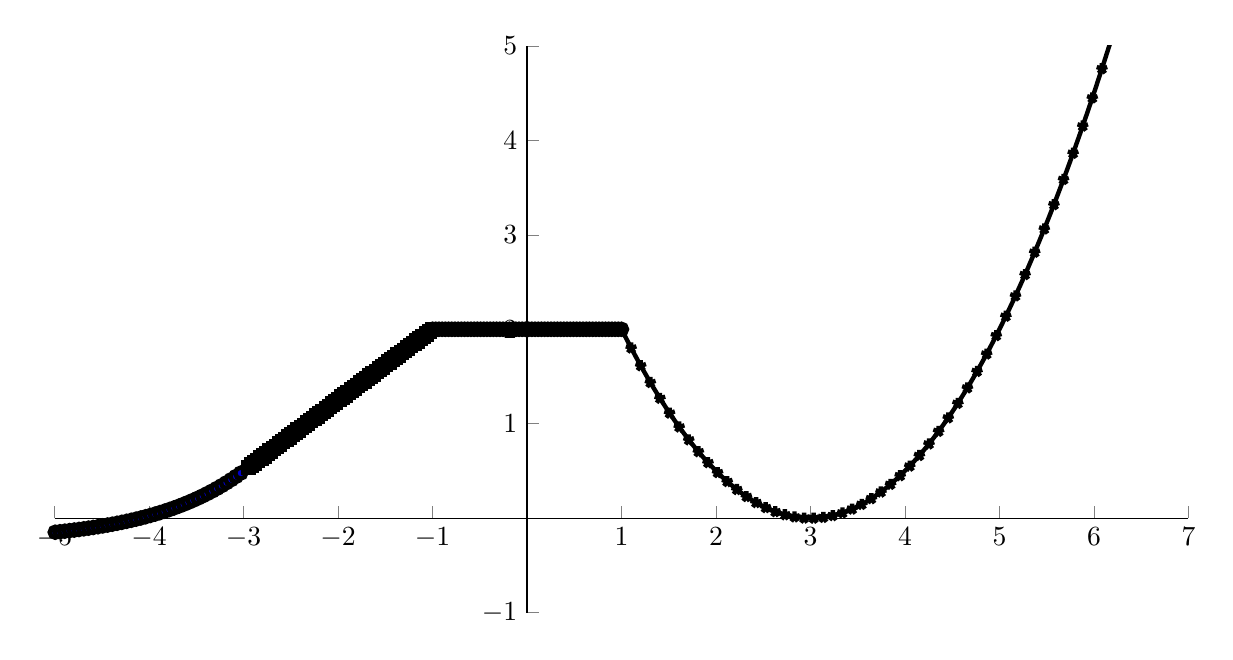
\begin{tikzpicture}[baseline=(current bounding box.north)]
        \begin{axis}[
        x=1.2cm,
        y=1.2cm,
        xmin=-5,
        xmax=7,
        ymin=-1,
        ymax=5,
        axis x line*=middle,
        axis y line*=middle,
        every axis plot/.append style={ultra thick},
        samples=60
        ]
        \addplot+[black, domain=-6:-3.03, restrict y to domain=-10:10] {e^(x+3+ln(3/4))-3/4+0.5};
        \addplot+[black, domain=-2.95:-1] {3/4*x+3/4+2};
        \addplot+[black, domain=-1:1] {2};
        \addplot+[black, domain=1:7] {1/2*(x-3)^2};
        \node at (-3,0.5) {$\circ$};
        \node at (-1,2) {\textbullet};
        \node at (1,2) {\textbullet};
        \end{axis}
        \end{tikzpicture}}
    
\end{document}